%using the old elsarticle cls by Elsevier
\documentclass[preprint,12pt,3p]{elsarticle}

%% Use the option review to obtain double line spacing
%% \documentclass[preprint,review,12pt]{elsarticle}

%% Use the options 1p,twocolumn; 3p; 3p,twocolumn; 5p; or 5p,twocolumn
%% for a journal layout:
%% \documentclass[final,1p,times]{elsarticle}
%% \documentclass[final,1p,times,twocolumn]{elsarticle}
%% \documentclass[final,3p,times]{elsarticle}
%% \documentclass[final,3p,times,twocolumn]{elsarticle}
%% \documentclass[final,5p,times]{elsarticle}
%% \documentclass[final,5p,times,twocolumn]{elsarticle}

%% if you use PostScript figures in your article
%% use the graphics package for simple commands
%% \usepackage{graphics}
%% or use the graphicx package for more complicated commands
%% \usepackage{graphicx}
%% or use the epsfig package if you prefer to use the old commands
%% \usepackage{epsfig}

%% The amssymb package provides various useful mathematical symbols
\usepackage{amssymb}
%% The amsthm package provides extended theorem environments
%% \usepackage{amsthm}

%% The lineno packages adds line numbers. Start line numbering with
%% \begin{linenumbers}, end it with \end{linenumbers}. Or switch it on
%% for the whole article with \linenumbers after \end{frontmatter}.
%% \usepackage{lineno}

%% natbib.sty is loaded by default. However, natbib options can be
%% provided with \biboptions{...} command. Following options are
%% valid:

%%   round  -  round parentheses are used (default)
%%   square -  square brackets are used   [option]
%%   curly  -  curly braces are used      {option}
%%   angle  -  angle brackets are used    <option>
%%   semicolon  -  multiple citations separated by semi-colon
%%   colon  - same as semicolon, an earlier confusion
%%   comma  -  separated by comma
%%   numbers-  selects numerical citations
%%   super  -  numerical citations as superscripts
%%   sort   -  sorts multiple citations according to order in ref. list
%%   sort&compress   -  like sort, but also compresses numerical citations
%%   compress - compresses without sorting
%%
%% \biboptions{comma,round}

% \biboptions{}


%\journal{Nuclear Physics B}
%journal{Numerical Practice Reports}
Numerical Practice Reports
\begin{document}

\begin{frontmatter}

\title{ \texttt{Numerical Practice 1 }}
%\tnotetext[label0]{This is only an example}


\author{Aakash Patil}
\address{aakash.patil@master.centralelille.fr}

%\ead[url]{author-one-homepage.com}

\begin{abstract}
1. Study of polynomial interpolation methods for Runge function and a Trigonometric function.  
\\
2. Study of interpolation error as a function of number of discretization points.
\end{abstract}

%\begin{keyword}
%% keywords here, in the form: keyword \sep keyword
%example \sep \LaTeX \sep template
%% MSC codes here, in the form: \MSC code \sep code
%% or \MSC[2008] code \sep code (2000 is the default)
%\end{keyword}

\end{frontmatter}

%%
%% Start line numbering here if you want
%%
% \linenumbers

%% main text
\section{Interpolation}
%\label{sec1}
Interpolation is used determine intermediate values between finite data points. The most common method used for this purpose is polynomial interpolation.$$ f(x) = a0 + a1 *x+a2 *x ^2 +------ + an *x^ n$$

For $n + 1$ data points, there is one and only one polynomial of order n that passes through all the points. For example, there is only one straight line (that is, a first-order polynomial) that connects two points. Similarly, only one parabola connects a set of three points. Polynomial interpolation consists of determining the unique nth-order polynomial that fits $n + 1$ data points. This polynomial then provides a relation to compute
intermediate values.


\section{Newton Divided Difference Interpolation Method}
There are a variety of alternative forms for expressing an interpolating
polynomial. Newton?s divided-difference interpolating polynomial is among the most popular and useful forms. 

The generalized equation to fit an nth-order polynomial to n + 1 data points.The nth-order polynomial as per Newton's method is:$$fn(x) = b0 + b1*(x-x 0 ) + -------- + bn*(x-x0)*(x-x1)--------(x-xn-1)$$

Data points can be used to evaluate the coefficients b 0 , b 1 , ---- , b n . For an nth-order polynomial, n + 1 data points are required: $[x 0 , f (x 0 )], [x 1 , f (x 1 )],--- , [x n , f (x n )]$. \\We use these data points and the following equations to evaluate the coefficients:\\  
$b 0 = f(x 0 )$\\
$b 1 = f [x 1 , x 0 ]$\\
$b 2 = f [x 2 , x 1 , x 0 ]$\\
-\\
-\\
-\\
$b n = f [x n , x n-1 , . . . , x 1 , x 0 ]$\\

where the bracketed function evaluations are finite divided differences. For example, the first finite divided difference is represented generally as $$f [x i , x j ] =
f (x i ) - f (x j ) / (x i - x j)$$
Similarly, the nth finite divided difference is$$f [x n , x n-1 , ---, x 1 , x 0 ] =
f [x n , x -1 , --- , x 1 ] - f [x n-1 , x n-2 ,-- , x 0 ]/(x n - x 0)$$

These coefficients can be evaluated and put in the equation to yield the interpolation polynomial.

%Sample text. Sample text. Citation of Einstein paper~\cite{Einstein}.

\section{Lagrange Interpolation Method}
The Lagrange interpolating polynomial is simply a reformulation of the Newton polynomial that avoids the computation of divided differences. It can be represented concisely as$$f(x)= \sum_{i=o}^{n} Li(x) *f (x i )$$
where$$Li(x)=\prod_{j=o,i}^{b} f(i)$$
For example, the linear version (n = 1) is$$f 1 (x) =(x - x 1)*f(x 0 )/(x 0 - x 1)+(x - x 0)*f(x 1 )/(x 1 - x 0)$$
the second-order version is$$f 2 (x) =(x - x 1 )*(x - x 2 )*f(x 0 )/(x 0 - x 1 )(x 0 - x 2 )+(x - x 0 )*(x - x 2 )*f(x 1 )/(x 1 - x 0 )(x 1 - x 2 )$$ $ +(x - x 0 )*(x - x 1 ) *f(x 2 )/(x 2 - x 0 )(x 2 - x 1 )$

\section{Code}
The code has been uploaded to \\

https://github.com/aakash30jan/ClassWork-TurbulenceMaster/tree/master/06-11-2017/src/
\newpage
\section{Results}
\subsection{Functions}
Following two functions were used to study polynomial interpolation:
\\Eq 1. $f(x)=1/(1+25x^{2})$     where     $x \varepsilon [-1,1] $\\
Eq 2. $f(x)=cos(x*\pi)$     where     $x \varepsilon [-1,1] $

\subsection{Plots}
 \begin{figure}
\centering
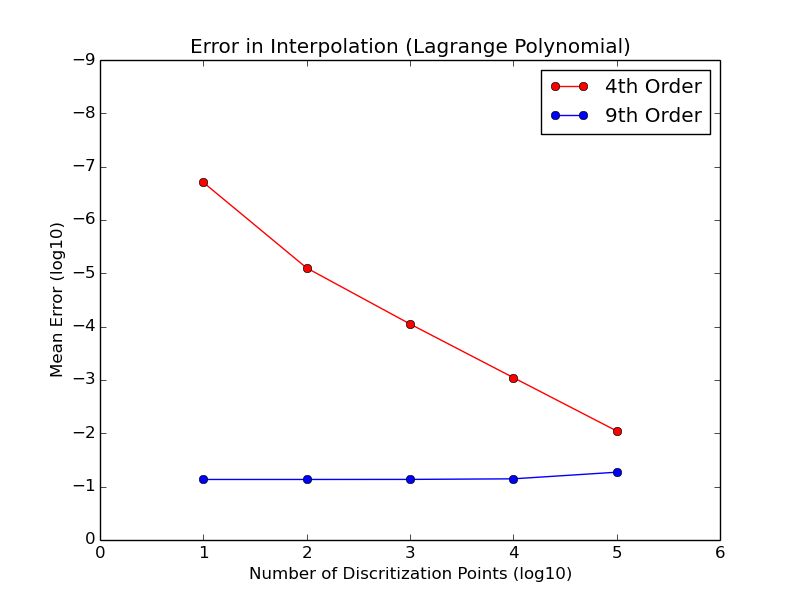
\includegraphics[width=0.7\linewidth]{eq1_lag.png}
\caption{Lagrange Interpolation Error for Equation 1 (4th and 9th order)}
\label{fig:eq1_lag}
\end{figure}


 \begin{figure}
\centering
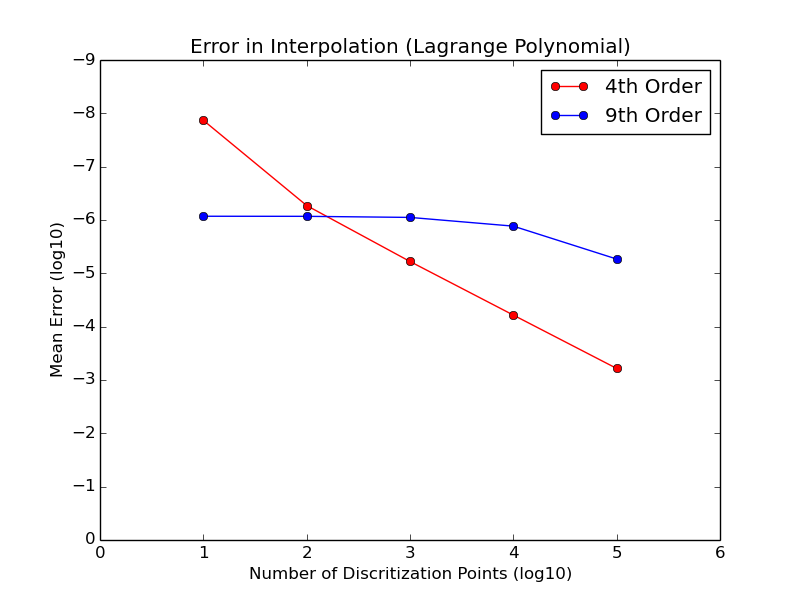
\includegraphics[width=0.7\linewidth]{eq2_lag.png}
\caption{Lagrange Interpolation Error for Equation 2 (4th and 9th order)}
\label{fig:eq2_lag}
\end{figure}


\begin{figure}
\centering
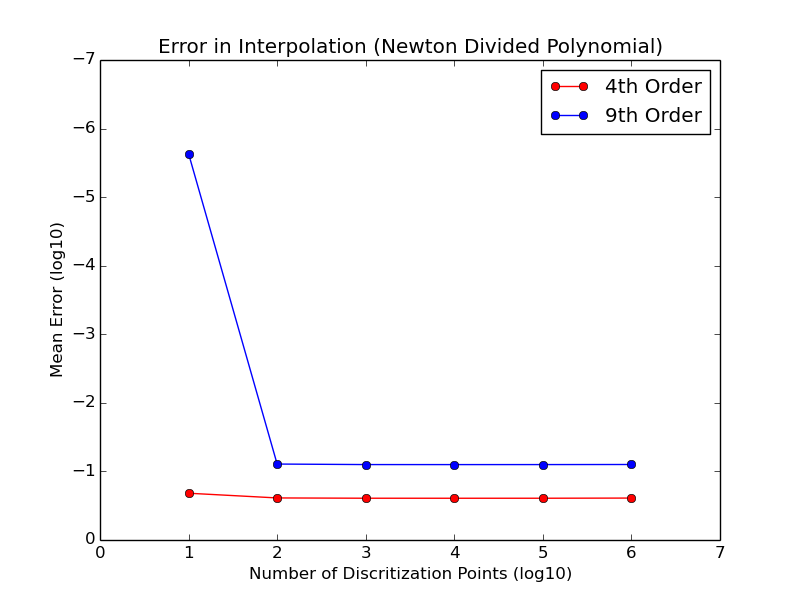
\includegraphics[width=0.7\linewidth]{eq1_newton.png}
\caption{Newton Interpolation Error for Equation 1 (4th and 9th order)}
\label{fig:eq1_newton}
\end{figure}


\begin{figure}
\centering
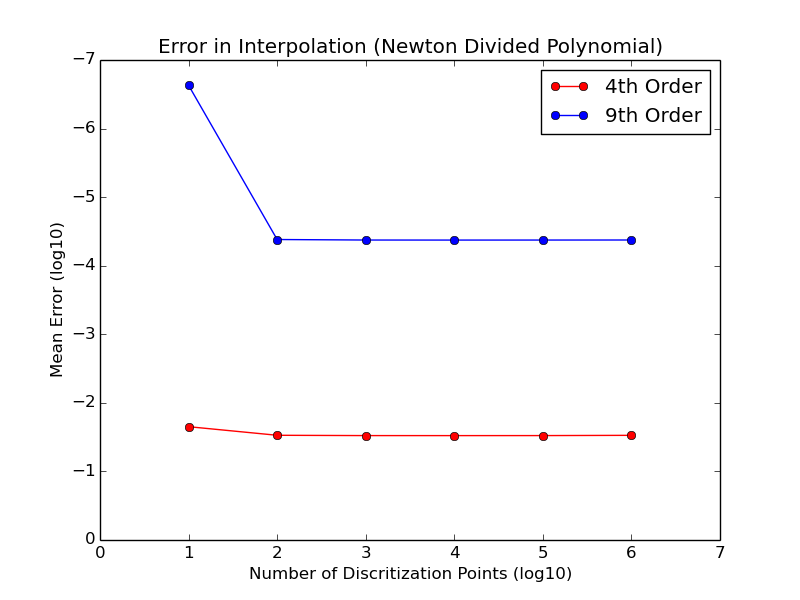
\includegraphics[width=0.7\linewidth]{eq2_newton.png}
\caption{Newton Interpolation Error for Equation 2 (4th and 9th order)}
\label{fig:eq2_newton}
\end{figure}



\begin{figure}
\centering
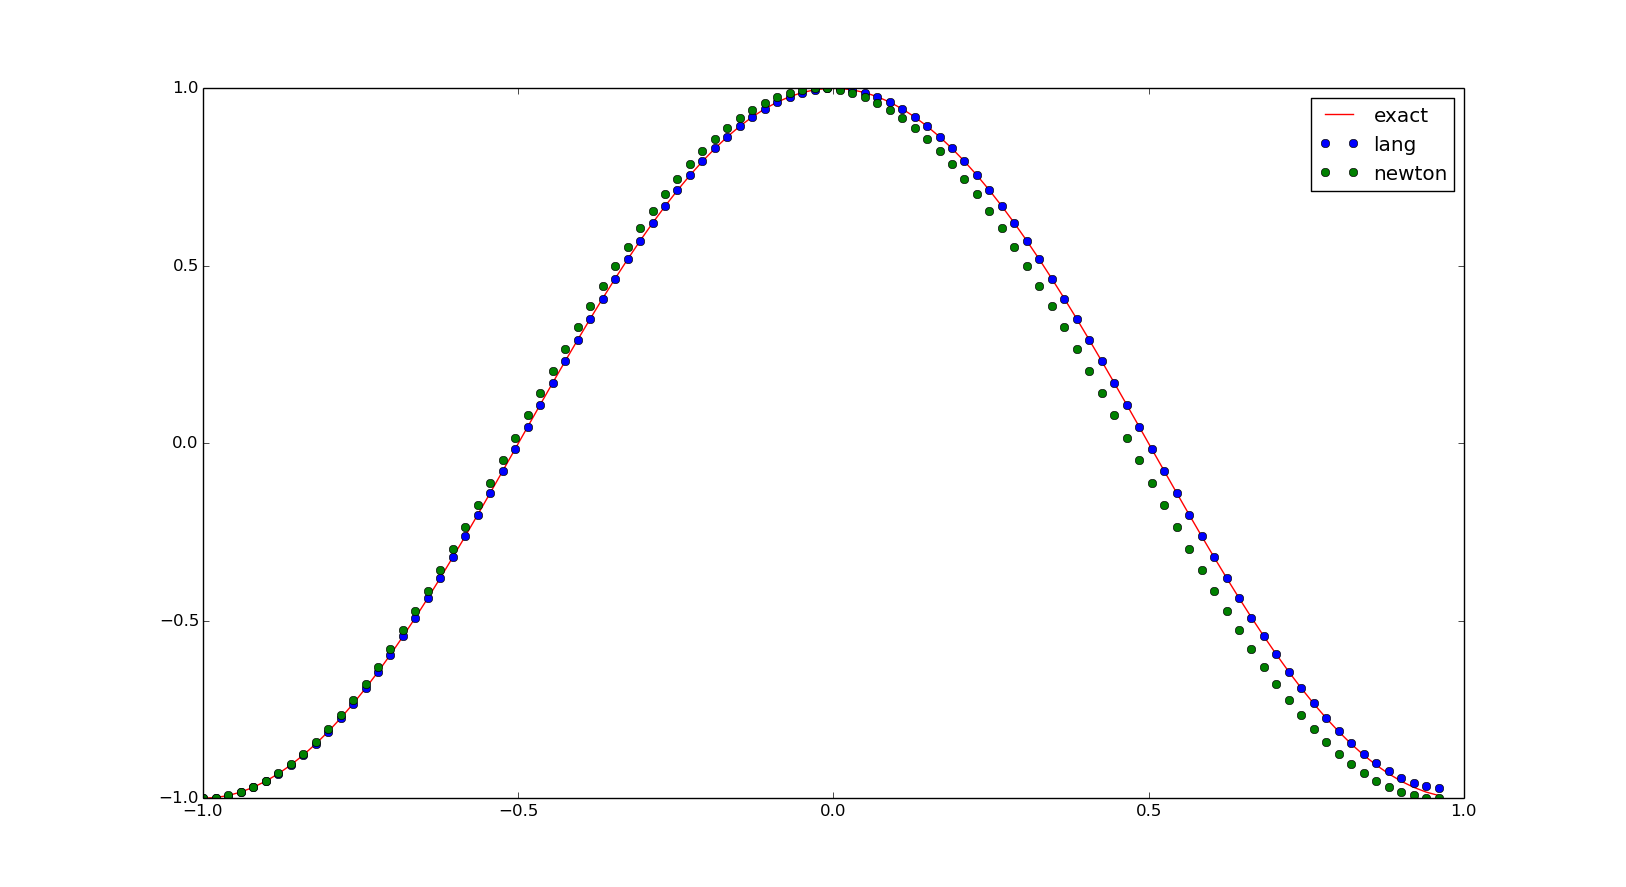
\includegraphics[width=0.8\linewidth]{eq2_n9_m100.png}
\caption{Comparison of interpolated points from 9th order polynomial for Equation 2}
\label{fig:eq2_n9_m100.png}
\end{figure}


%% The Appendices part is started with the command \appendix;
%% appendix sections are then done as normal sections
%\appendix

%\section{Section in Appendix}
%\label{appendix-sec1}

%Sample text. Sample text. Sample text. Sample text. Sample text. Sample text. 
%Sample text. Sample text. Sample text. Sample text. Sample text. Sample text. 
%Sample text. 

%% References
%%
%% Following citation commands can be used in the body text:
%% Usage of \cite is as follows:
%%   \cite{key}         ==>>  [#]
%%   \cite[chap. 2]{key} ==>> [#, chap. 2]
%%

%% References with bibTeX database:

%\bibliographystyle{elsarticle-num}
% \bibliographystyle{elsarticle-harv}
% \bibliographystyle{elsarticle-num-names}
% \bibliographystyle{model1a-num-names}
% \bibliographystyle{model1b-num-names}
% \bibliographystyle{model1c-num-names}
% \bibliographystyle{model1-num-names}
% \bibliographystyle{model2-names}
% \bibliographystyle{model3a-num-names}
% \bibliographystyle{model3-num-names}
% \bibliographystyle{model4-names}
% \bibliographystyle{model5-names}
% \bibliographystyle{model6-num-names}

%\bibliography{sample}


\end{document}

%%
%% End of file
